%%%%%%%% ICML 2025 EXAMPLE LATEX SUBMISSION FILE %%%%%%%%%%%%%%%%%

\documentclass{article}

% Recommended, but optional, packages for figures and better typesetting:
\usepackage{microtype}
\usepackage{graphicx}
\usepackage{subfigure}
\usepackage{booktabs} % for professional tables

% hyperref makes hyperlinks in the resulting PDF.
% If your build breaks (sometimes temporarily if a hyperlink spans a page)
% please comment out the following usepackage line and replace
% \usepackage{icml2025} with \usepackage[nohyperref]{icml2025} above.
\usepackage{hyperref}


% Attempt to make hyperref and algorithmic work together better:
\newcommand{\theHalgorithm}{\arabic{algorithm}}

% Use the following line for the initial blind version submitted for review:
\usepackage[accepted]{icml2025}

% If accepted, instead use the following line for the camera-ready submission:
% \usepackage[accepted]{icml2025}

% For theorems and such
\usepackage{amsmath}
\usepackage{amssymb}
\usepackage{mathtools}
\usepackage{amsthm}

% if you use cleveref..
\usepackage[capitalize,noabbrev]{cleveref}

%%%%%%%%%%%%%%%%%%%%%%%%%%%%%%%%
% THEOREMS
%%%%%%%%%%%%%%%%%%%%%%%%%%%%%%%%
\theoremstyle{plain}
\newtheorem{theorem}{Theorem}[section]
\newtheorem{proposition}[theorem]{Proposition}
\newtheorem{lemma}[theorem]{Lemma}
\newtheorem{corollary}[theorem]{Corollary}
\theoremstyle{definition}
\newtheorem{definition}[theorem]{Definition}
\newtheorem{assumption}[theorem]{Assumption}
\theoremstyle{remark}
\newtheorem{remark}[theorem]{Remark}

% Todonotes is useful during development; simply uncomment the next line
%    and comment out the line below the next line to turn off comments
%\usepackage[disable,textsize=tiny]{todonotes}
\usepackage[textsize=tiny]{todonotes}


% The \icmltitle you define below is probably too long as a header.
% Therefore, a short form for the running title is supplied here:
\icmltitlerunning{Submission and Formatting Instructions for ICML 2025}

\begin{document}

\twocolumn[
\icmltitle{Implementing and Improving Show, Attend, and Tell }

% It is OKAY to include author information, even for blind
% submissions: the style file will automatically remove it for you
% unless you've provided the [accepted] option to the icml2025
% package.

% List of affiliations: The first argument should be a (short)
% identifier you will use later to specify author affiliations
% Academic affiliations should list Department, University, City, Region, Country
% Industry affiliations should list Company, City, Region, Country

% You can specify symbols, otherwise they are numbered in order.
% Ideally, you should not use this facility. Affiliations will be numbered
% in order of appearance and this is the preferred way.
\icmlsetsymbol{equal}{*}

\begin{icmlauthorlist}
\icmlauthor{Isabella Mercado}{sch}
\end{icmlauthorlist}

\icmlaffiliation{sch}{University of Chicago, Chicago, USA}

\icmlcorrespondingauthor{Isabella Mercado}{imercado@uchicago.edu}

% You may provide any keywords that you
% find helpful for describing your paper; these are used to populate
% the "keywords" metadata in the PDF but will not be shown in the document
\icmlkeywords{Machine Learning, ICML}

\vskip 0.3in
]

% this must go after the closing bracket ] following \twocolumn[ ...

% This command actually creates the footnote in the first column
% listing the affiliations and the copyright notice.
% The command takes one argument, which is text to display at the start of the footnote.
% The \icmlEqualContribution command is standard text for equal contribution.
% Remove it (just {}) if you do not need this facility.

%\printAffiliationsAndNotice{}  % leave blank if no need to mention equal contribution
\printAffiliationsAndNotice{\icmlEqualContribution} % otherwise use the standard text.

\begin{abstract}
This report presents an implementation and architectural improvements of the "Show, Attend and Tell" model for neural image caption generation with visual attention. I begin with a brief overview of the original architecture, which pioneered the use of attention mechanisms in image captioning. I then detail my implementation of this model, highlighting both similarities and differences with the original paper's approach. Furthermore, I describe several architectural enhancements made to the original implementation, including improvements to the encoder-decoder framework, attention mechanism refinements, and training methodology optimizations. My modifications aim to enhance the model's performance in generating accurate image descriptions while maintaining computational efficiency.
\end{abstract}

\section{Introduction}

The task of automatically generating natural language descriptions for images is a complex, but important challenge in computer vision and natural language processing. The seminal "Show, Attend and Tell" paper by Xu et al. (2015) introduced a novel approach to image captioning by integrating attention mechanisms with latent representations of images. The authors demonstrated both qualitatively, through visualizations of attention, and quantitatively, through BLEU Score measurements, the utility in guiding a model's focus to specific, relevant regions of an image when generating each word of a caption.

The original architecture combined a convolutional neural network (CNN) for image feature extraction with a long-short term memory network (LSTM) for textual sequence generation. As opposed to utilizing the feature vectors outputted by the final fully-connected layer of a CNN similar to previous approaches, the authors extract features from a lower convolutional network to retain spatial information that can leveraged by the attention mechanism. In this paper, I replicate, train and evaluate the core architecture described in the original paper in order to establish a baseline reference point. From there, I extend beyond the methodology implemented in the original paper, improving the encoder, decoder, and training architectures to ultimately drive higher performance than the original paper. 

\section{Original Implementation Analysis}

My base implementation follows the core architecture described in the original paper, which I trained and validated on the 2014 Microsoft COCO (Common Objects in Context) dataset with 82,783 images in my training set and 40,504 images in my validation set. 

\subsection{Encoder Architecture}

The original paper employed a modified VGG-16 network as the encoder, removing the final fully connected layer to maintain spatial information in the feature maps. My base implementation replicates their work with a similarly modified VGG-19 network with a marginal difference of 3 convolutional layers differentiating the two.

The features extracted from the lower convolutional layer are representations of the inputted image that correspond mathematically with:

\begin{equation}
\textbf{a} = \{a_1, \ldots, a_L\}, a_i \in \mathbb{R}^D
\end{equation}
where $\textbf{a}$ represents the set of $L$ annotation vectors, each encoding a portion of the image. For VGG-19, $L = 196$ (corresponding to a $14 \times 14$ spatial grid) and $D = 512$.

\subsection{Attention Mechanism}

The attention mechanism in my implementation closely follows the soft attention approach described in the paper. For each hidden state $h_t$ of the decoder, attention weights $\alpha_{ti}$ are computed for each spatial location $i$ in the image feature map. These attention weights then serve to calculate the context vector $\hat{z}_t$, which is a weighted sum of annotation vectors:

\begin{align}
e_{ti} &= f_{att}(a_i, h_{t-1}) \\
\alpha_{ti} &= \frac{\exp(e_{ti})}{\sum_{j=1}^{L} \exp(e_{tj})} \\
\hat{z}_t &= \phi(\{a_i\}, \{\alpha_i\}) = \sum_{i=1}^{L} \alpha_{ti} a_i
\end{align}

Although the details were not explicitly identified in the original paper, my attention block inputs the previous hidden state and current annotation vector into respective linear layers. It concatenates the results and feeds to a  tanh function to generate $e_{ti}$. 

\begin{equation}
f_{att} = \tanh(W_{ht} h_{t-1} + b_{ht} + W_{a} a_i + b_{ai})
\end{equation}

Additionally, my implementation includes a gating scalar $\beta_t$ that modulates the context vector before it is fed into the LSTM, allowing the model to adaptively weight the importance of context vector at each time step.

\begin{equation}
\beta_t = \sigma(W_{\beta} h_{t-1} + b_{\beta})
\end{equation}

Although this adaptive attention technique was not mentioned in the original paper, but is recognized to improve performance.

\subsection{Decoder Architecture}

The decoder utilizes an LSTM network to produce captions by sequentially generating words given the context vector, previous hidden state, and previously generated words. At each time step $t$, the model computes:

\begin{align}
i_t &= \sigma(W_{ix} x_t + W_{ih} h_{t-1} + W_{ic} c_{t-1} + b_i) \\
f_t &= \sigma(W_{fx} x_t + W_{fh} h_{t-1} + W_{fc} c_{t-1} + b_f) \\
o_t &= \sigma(W_{ox} x_t + W_{oh} h_{t-1} + W_{oc} c_{t-1} + b_o) \\
g_t &= \tanh(W_{gx} x_t + W_{gh} h_{t-1} + b_g) \\
c_t &= f_t \odot c_{t-1} + i_t \odot g_t \\
h_t &= o_t \odot \tanh(c_t)
\end{align}

where $x_t$ is the concatenation of the word embedding and the gated context vector $\beta_t \cdot \hat{z}_t$. Just as in the original paper, the output word probability is calculated using a deep output layer.

\section{Architectural Improvements}

My enhanced implementation includes several architectural improvements which serve to increase the efficiency and accuracy of my model.
    
\subsection{Modern CNN} My advanced implementation leverages the final convolutional layer of the ResNet-101 network (obtained by removing the final layer and penultimate average pooling layer). Although both were trained on the substantial ImageNet dataset, the VGG model utilizes a simple sequential structure with 16 convolutional layers and 3 fully connnected layers, while the ResNet has 101 layers with residual blocks that allow information to bypass layers. As a result the ResNet is computationally more efficient and accurate, driving superior gradient flow and feature extraction. Mathematically, for an input image $I \in \mathbb{R}^{H \times W \times 3}$, my ResNet101 encoder produces feature vectors $F \in \mathbb{R}^{h \times w \times d}$ where $h=7, w=7, d=2048$. These features are then reshaped to $F' \in \mathbb{R}^{49 \times 2048}$ before being passed to the LSTM.

\subsection{Length-aware batch processing} The decoder sorts the ground-truth captions by decreasing length and continues generating captions only for samples whose current timestep is less than the length of their ground-truth caption. This technique ensures that each sample in a batch is processed only for the necessary number of timesteps, improving the efficiency of batch training for variable-length sequences. By focusing computation on active sequences, the model avoids unnecessary processing of completed captions, optimizing both computational resources and training time.

\subsection{CNN fine-tuning} The original implementation as well as that analyzed throughout my paper uses a fixed pre-trained CNN, however, my repository additionally integrates the option to fine-tune the final convolutional blocks of a specified CNN model. This could enable the CNN model to adapt the visual features to the specific task of image captioning and improve the accuracy of my entire pipeline. 

\section{Training Methodology Improvements}

The original paper named multiple training techniques such as dropout, early stopping based on BLEU score, and evaluating models based on BLEU scores calculated on the validation set. My base model leverages all of these techniques, however, my enhanced version uses a variety of more advanced techniques to improve model performance.

\subsection{Label Smoothing Loss}

Label smoothing is a regularization technique used to improve the generalization of neural networks. Instead of assigning a probability of 1 to the correct class and 0 to all others, label smoothing assigns a slightly lower probability to the correct class and distributes the remaining probability mass across the other classes. Unlike standard cross-entropy loss, label smoothing discourages the model from assigning extremely high probabilities to training examples, making it less susceptible to overfitting the training data and better at generalizations.

In my implementation, I use a label smoothing factor of 0.1. The loss is calculated as a combination of the negative log-likelihood of the correct class and the average log-likelihood of all classes, weighted by the smoothing factor. This is mathematically represented as:

\begin{equation}
\mathcal{L} = (1 - \epsilon) \cdot \text{NLL} + \epsilon \cdot \text{Smooth\_Loss}
\end{equation}

where \(\epsilon\) is the smoothing factor, \(\text{NLL}\) is the negative log-likelihood of the correct class, and \(\text{Smooth\_Loss}\) is the average log-likelihood of all classes.
    
\subsection{Teacher forcing} Teacher forcing is a training technique used in sequence-to-sequence models, such as those used for language generation tasks. During training, at each step of sequence generation, the model receives the correct token from the ground-truth sequence as input for the next step, instead of using the token it predicted in the previous step. By providing the correct context at each step, teacher forcing helps the model learn the correct sequence patterns more quickly, leading to faster convergence, greater stability, and improved learning.
    
\subsection{Gradient clipping} To prevent exploding gradients, I applied gradient clipping:
    
\begin{equation}
\nabla_{\theta} \mathcal{L} = \min \left( \max \left( \nabla_{\theta} \mathcal{L}, -c \right), c \right)
\end{equation}

where $c$ is the clipping threshold.
    
\subsection{Learning rate scheduling} I implemented step decay for the learning rate:
    
\begin{equation}
\eta_{epoch} = \eta_{0} \cdot \gamma^{\lfloor \frac{epoch}{step\_size} \rfloor}
\end{equation}

where $\gamma$ is the decay factor and $step\_size$ is the number of epochs after which to decay the learning rate.

\subsection{Regularization} I introduced dropout in the decoder to prevent overfitting. During training, dropout randomly sets a fraction of the neurons in a layer to zero at each forward pass. This fraction is determined by a hyperparameter called the dropout rate, typically denoted as p:
    
\begin{align}
p_t &= \text{dropout}(h_t, p) \\
y_t &= \text{softmax}(W_o p_t + b_o)
\end{align}

Dropout helps prevent overfitting to the training data and improve the generalizability to new data. 


\section{Results and Discussion}

\begin{figure}[htbp]
    \centering
    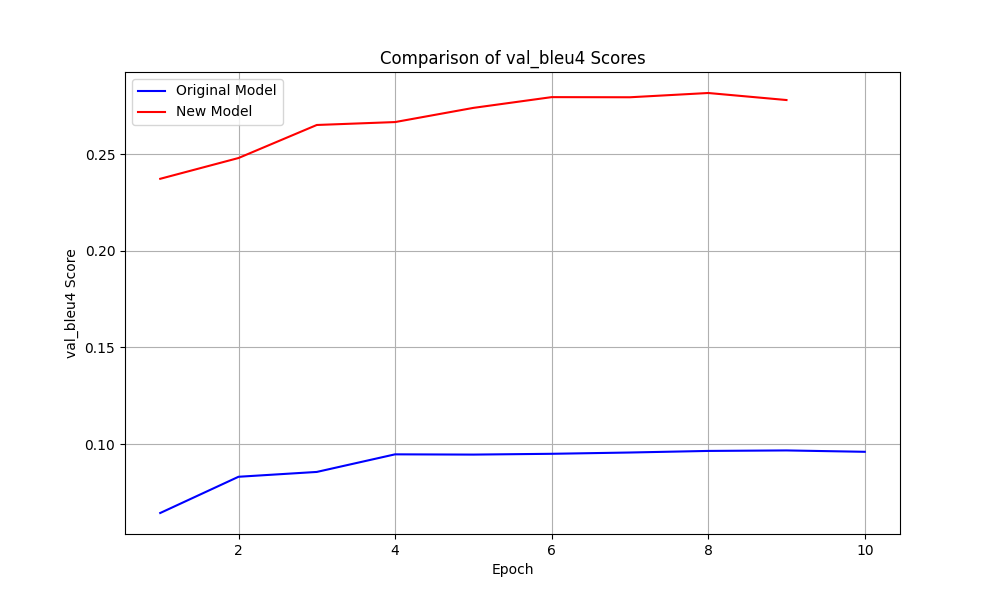
\includegraphics[width=\linewidth]{val_bleu4_comparison.png}
    \caption{BLEU-4 Score Comparison.}
    \label{fig:example}
\end{figure}

As visible in Figure 1, the previously described architectural improvements drove a remarkable improvement between the baseline model created based on the original paper's architecture and my enhanced model. The baseline model reached a peak BLEU-4 score of 0.08, while the enhanced model outperformed the original model with a BLEU-4 score of 28.77. Similar advances are seen in BLEU-1, BLEU-2, and BLEU-3 (See Figure 2 in Appendix). The most remarkable feature of this improved architecture were the efficiency gains in training time.

I trained the baseline model for 10 epochs and the enhanced model for 9 epochs each on an H100 GPU. I stopped training the enhanced model prior to 10 epochs because, as reported by my early stopping indicator, the BLEU-4 stopped improving by epoch 8. The enhanced model took about 4 hours to train, significantly less than the 3 day period the original paper trained their model for, while still outperforming the paper's BLEU-4 score of 24.3. My baseline model took two hours longer with significantly worse performance. While observing marginal performance gains from including the RESNET-101 network and many of the other advanced techniques, training efficiency and quantitative model performance significantly improved from the incorporation of teacher forcing. However, I did not measure the qualitative performance of an enhanced model without teacher forcing.

The increase in BLEU scores correspond to significant qualitative improvements in generated image captions. The baseline model outputted incoherent caption with frequent word repetitions, while the enhanced model produced highly descriptive captions for the same validation set images (See Figures 7 and 8 in Appendix). The same qualitative improvements are observed in the representations I generated of what the model "attended" to whilst generating a particular word in a caption (See Figures 3-6 in the Appendix). These results indicate the remarkable improvements that can be made over the original paper's model with the incorporation of incorporation of enhanced architecture and training methodologies. 

\section{Conclusion}

I have presented an implementation and enhancement of the "Show, Attend and Tell" model for image captioning. My modifications to the encoder-decoder architecture, attention mechanism, and training methodology address several limitations of the original implementation while maintaining the core insights of the original paper.

The flexibility to use modern CNN architectures, the improved decoder model, and the enhanced training procedures collectively represent a significant advancement over the base implementation. These improvements not only enhance model performance but also improve training efficiency and stability.

Future work could explore the integration of more advanced attention mechanisms or testing the encoder fine-tuning paradigm included, but not tested, in this paper's associated repository.

\bibliography{example_paper}
\bibliographystyle{icml2025}
K. Xu, J. Ba, R. Kiros, K. Cho, A. Courville, R. Salakhudinov, R. Zemel, and Y. Bengio. Show, attend and tell: Neural image caption generation with visual attention. In International Conference on Machine Learning, pp. 2048–2057. PMLR, 2015.

A. C. Wong. Show-Attend-and-Tell. GitHub repository, 2017. URL https://github.com/AaronCCWong/Show-Attend-and-Tell.



%%%%%%%%%%%%%%%%%%%%%%%%%%%%%%%%%%%%%%%%%%%%%%%%%%%%%%%%%%%%%%%%%%%%%%%%%%%%%%%
%%%%%%%%%%%%%%%%%%%%%%%%%%%%%%%%%%%%%%%%%%%%%%%%%%%%%%%%%%%%%%%%%%%%%%%%%%%%%%%
% APPENDIX
%%%%%%%%%%%%%%%%%%%%%%%%%%%%%%%%%%%%%%%%%%%%%%%%%%%%%%%%%%%%%%%%%%%%%%%%%%%%%%%
%%%%%%%%%%%%%%%%%%%%%%%%%%%%%%%%%%%%%%%%%%%%%%%%%%%%%%%%%%%%%%%%%%%%%%%%%%%%%%%
\newpage
\appendix
\onecolumn
\section{Appendix.}

\begin{figure}[htbp]
    \centering
    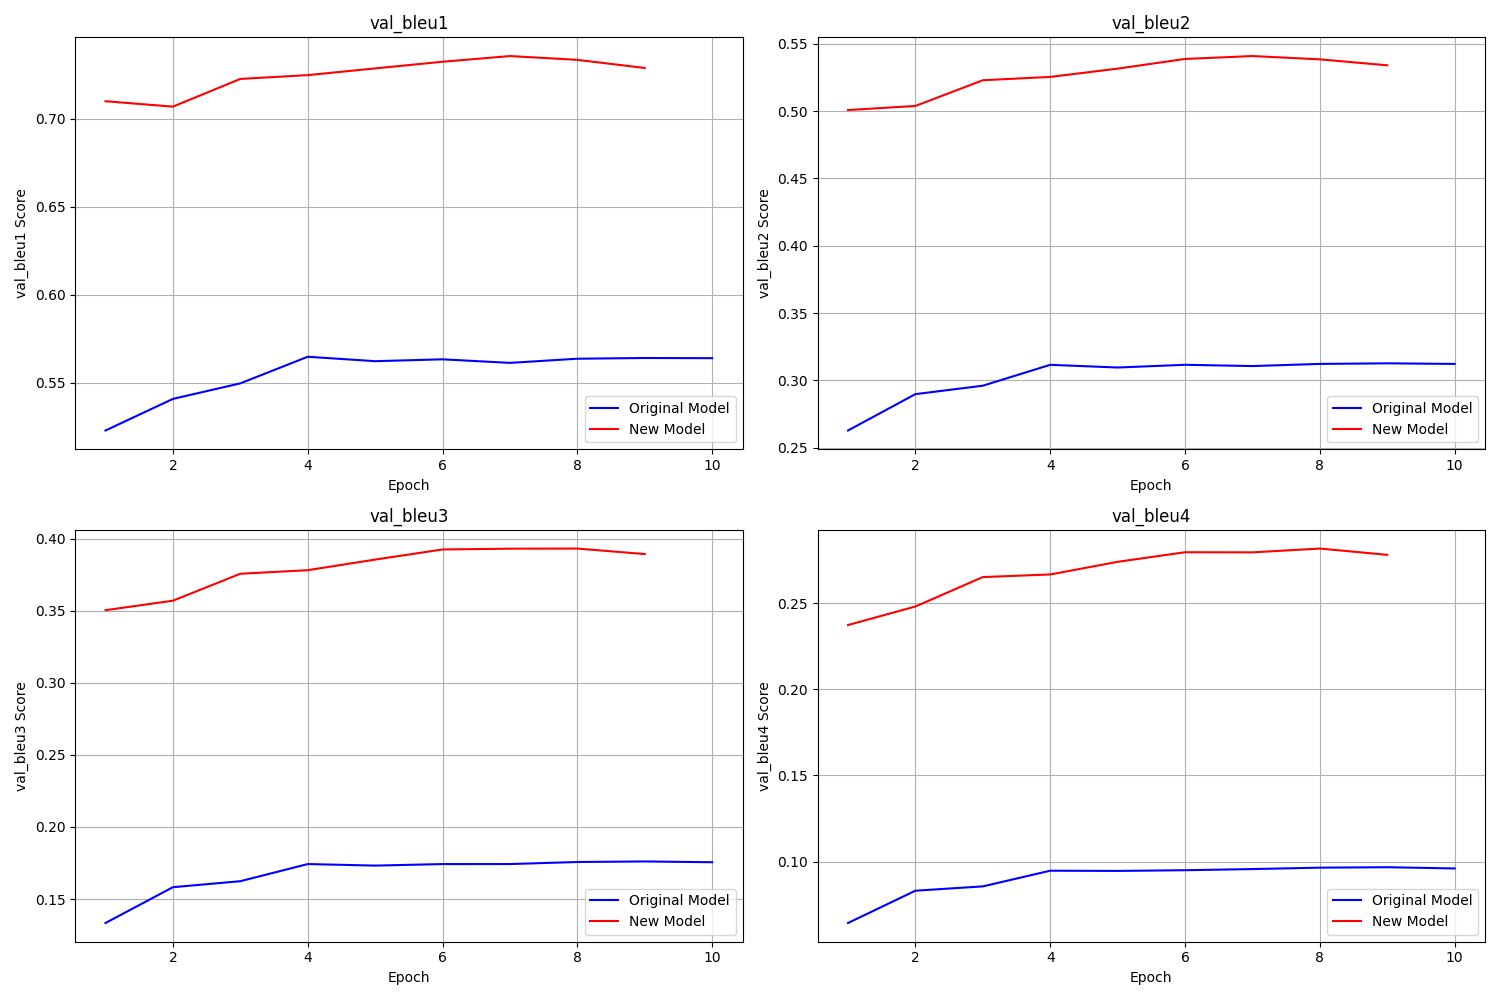
\includegraphics[width=\linewidth]{all_bleu_comparison.png}
    \caption{Comparing BLEU-1, BLEU-2, BLEU-3, \& BLEU-4 scores across epochs for baseline and enhanced model.}
    \label{fig:example}
\end{figure}

\begin{figure}[htbp]
    \centering
    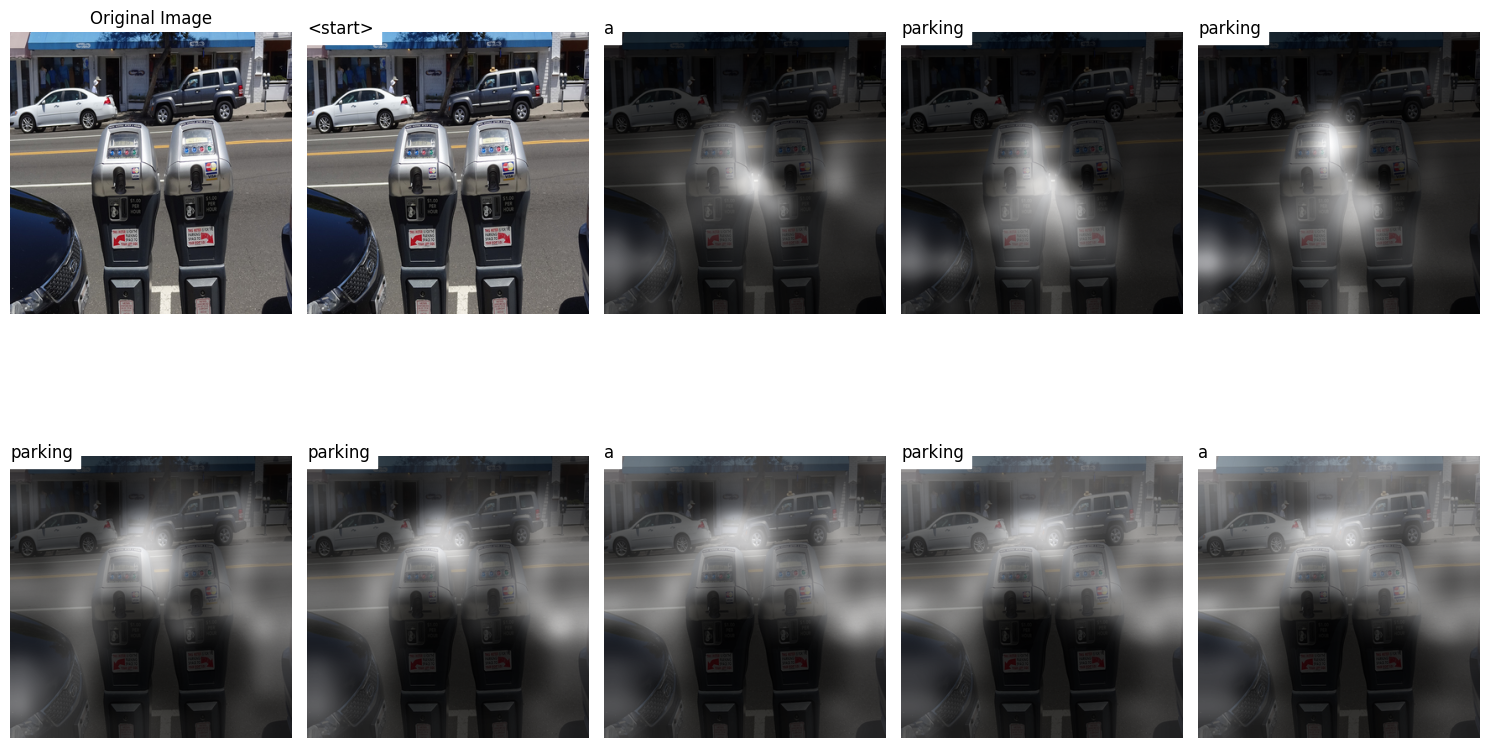
\includegraphics[width=\linewidth]{COCO_train2014_000000476761.jpg_caption.png}
    \caption{Training Set Image for Baseline Model.}
    \label{fig:example}
\end{figure}

\begin{figure}[htbp]
    \centering
    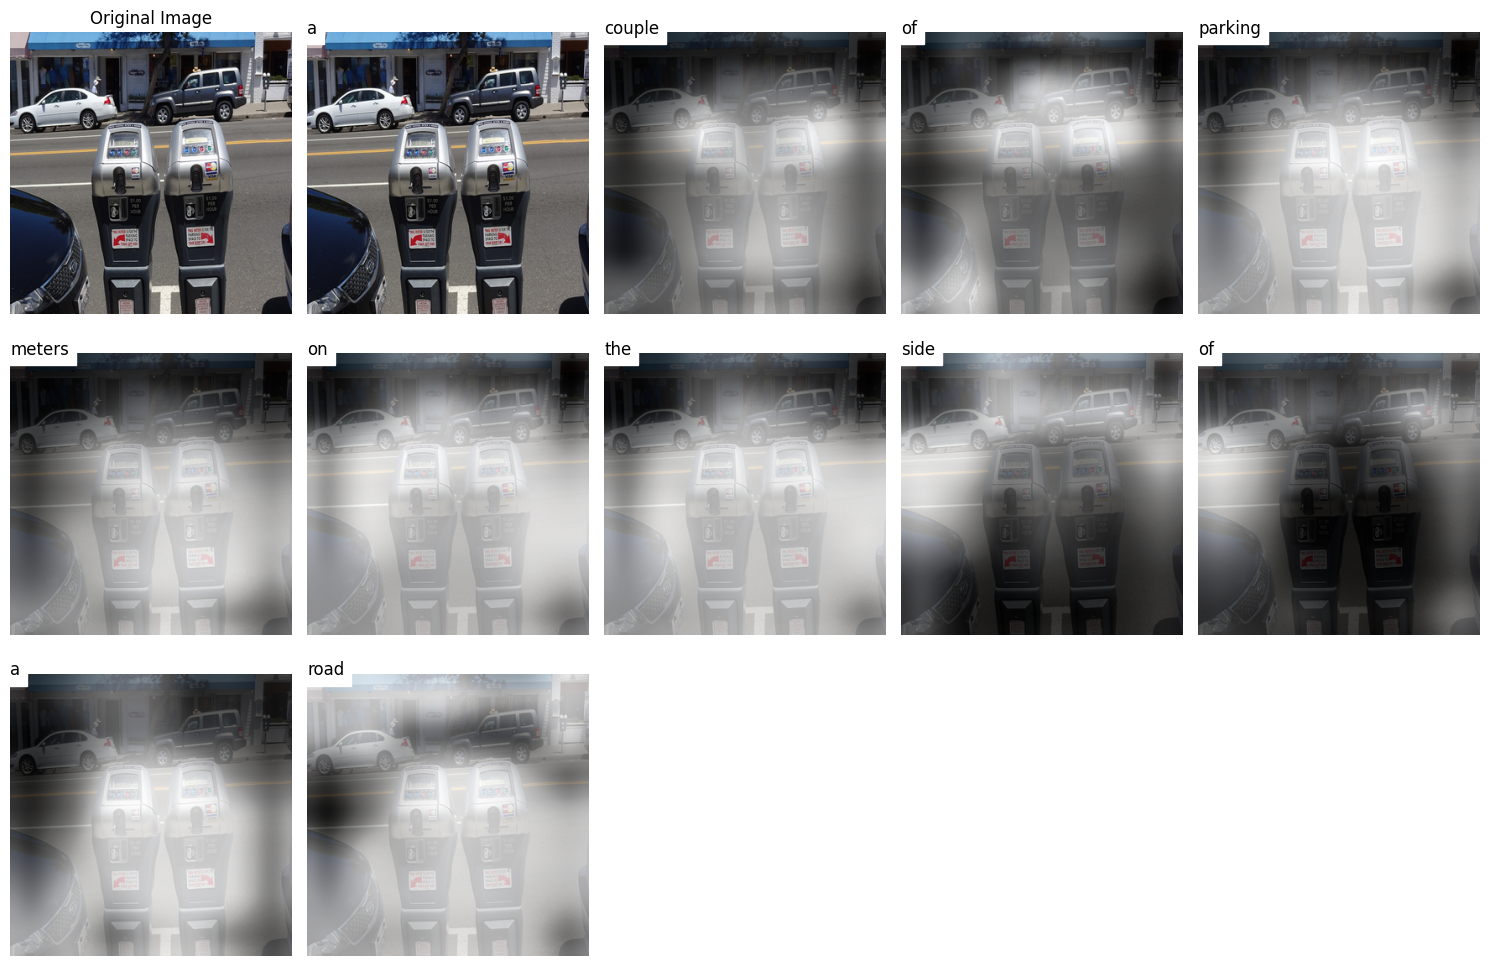
\includegraphics[width=\linewidth]{COCO_train2014_000000476761_caption.png}
    \caption{Training Set Image for Enhanced Model.}
    \label{fig:example}
\end{figure}

\begin{figure}[htbp]
    \centering
    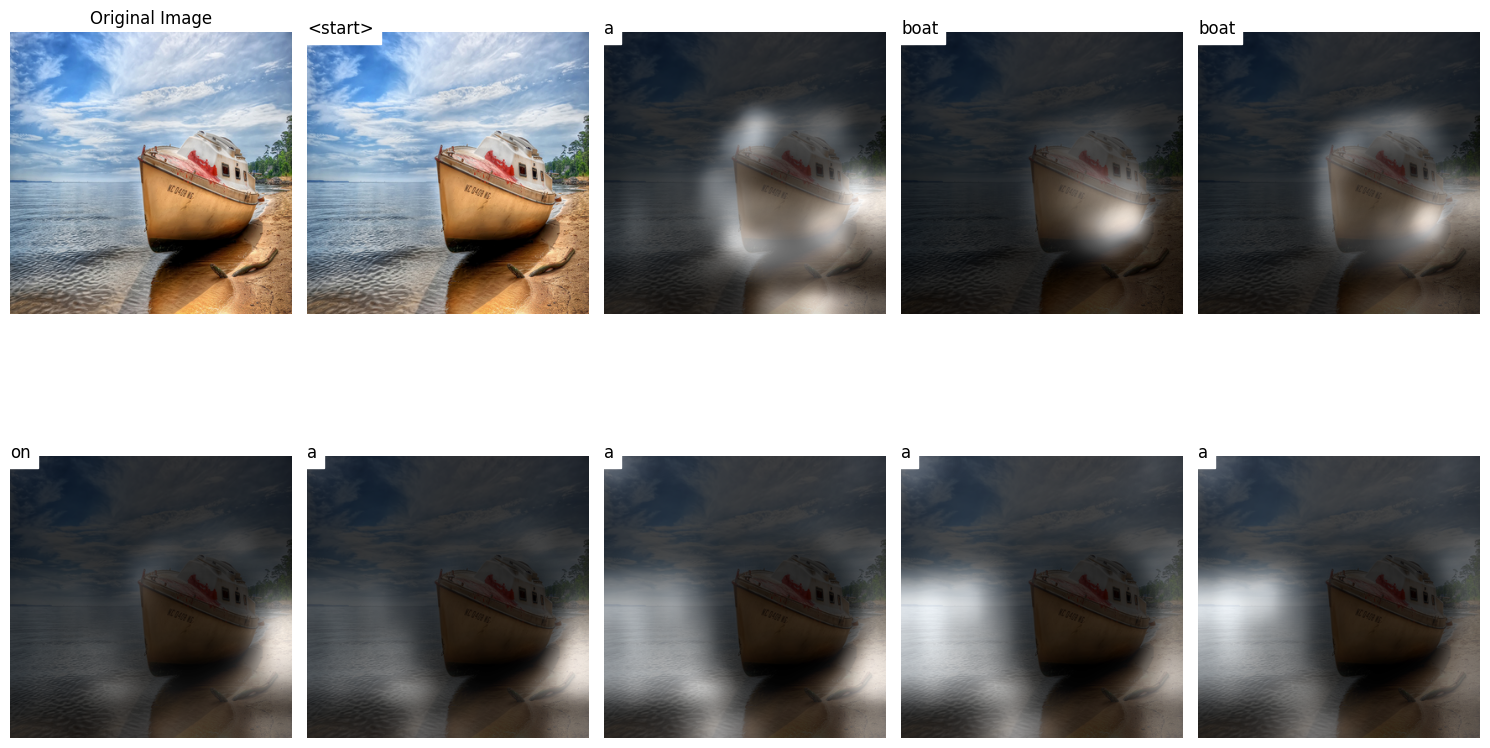
\includegraphics[width=\linewidth]{COCO_val2014_000000354744_caption.png}
    \caption{Validation Set Image for Baseline Model.}
    \label{fig:example}
\end{figure}

\begin{figure}[htbp]
    \centering
    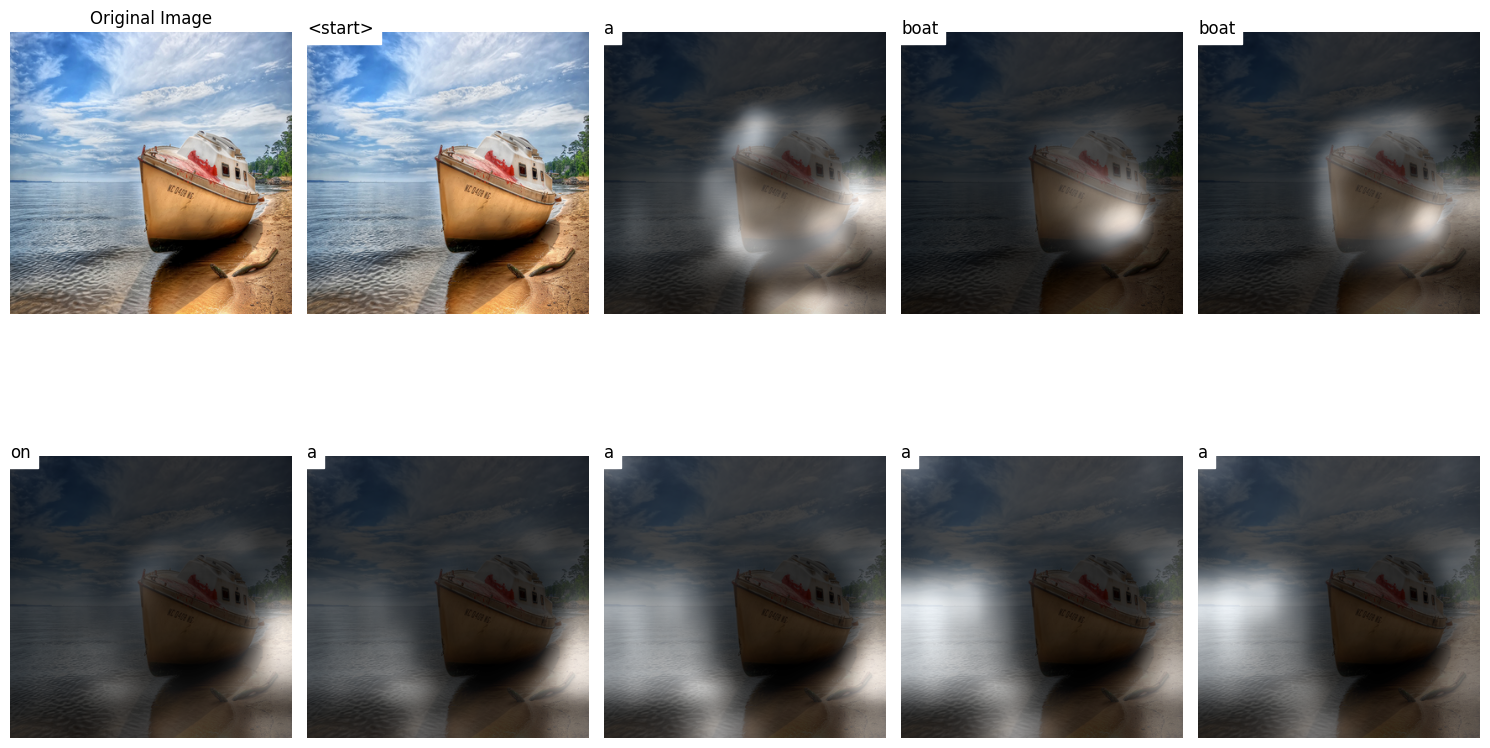
\includegraphics[width=\linewidth]{COCO_val2014_000000354744.jpg_caption.png}
    \caption{Validation Set Image for Enhanced Model.}
    \label{fig:example}
\end{figure}

\begin{figure}[htbp]
    \centering
    \includegraphics[width=\linewidth]{Screenshot 2025-03-15 at 10.24.36 PM.png}
    \caption{Validation Set Captions for Baseline Model.}
    \label{fig:example}
\end{figure}

\begin{figure}[htbp]
    \centering
    \includegraphics[width=\linewidth]{Screenshot 2025-03-15 at 10.10.03 PM.png}
    \caption{Validation Set Captions for Enhanced Model.}
    \label{fig:example}
\end{figure}

%%%%%%%%%%%%%%%%%%%%%%%%%%%%%%%%%%%%%%%%%%%%%%%%%%%%%%%%%%%%%%%%%%%%%%%%%%%%%%%
%%%%%%%%%%%%%%%%%%%%%%%%%%%%%%%%%%%%%%%%%%%%%%%%%%%%%%%%%%%%%%%%%%%%%%%%%%%%%%%


\end{document}


% This document was modified from the file originally made available by
% Pat Langley and Andrea Danyluk for ICML-2K. This version was created
% by Iain Murray in 2018, and modified by Alexandre Bouchard in
% 2019 and 2021 and by Csaba Szepesvari, Gang Niu and Sivan Sabato in 2022.
% Modified again in 2023 and 2024 by Sivan Sabato and Jonathan Scarlett.
% Previous contributors include Dan Roy, Lise Getoor and Tobias
% Scheffer, which was slightly modified from the 2010 version by
% Thorsten Joachims & Johannes Fuernkranz, slightly modified from the
% 2009 version by Kiri Wagstaff and Sam Roweis's 2008 version, which is
% slightly modified from Prasad Tadepalli's 2007 version which is a
% lightly changed version of the previous year's version by Andrew
% Moore, which was in turn edited from those of Kristian Kersting and
% Codrina Lauth. Alex Smola contributed to the algorithmic style files.
